\section{Sklepanje}
\subsection{Bayesovske mreze}
Baye. mreza = Usmerjen graf, kjer so podane zahtevane verjetnosti:
\begin{itemize}[leftmargin=*,topsep=0pt,noitemsep]
    \item Za vozlisca \textbf{brez starsev} verjetnosti $P(v_i)$
    \item Za vozlisca z \textbf{starsi} pogojne verjetnosti vseh kombinacij starsev
\end{itemize}
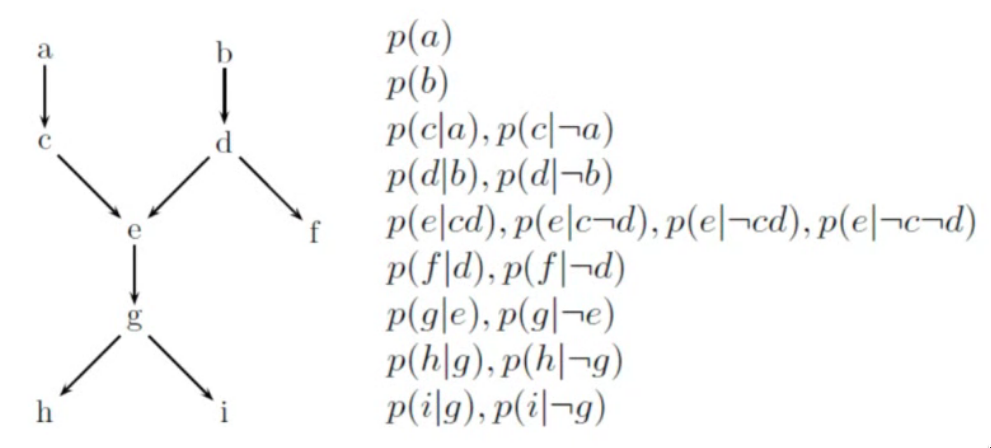
\includegraphics[width=6cm]{images/bayesovska_mreza.png}
Pravila verjetnostnega sklepanja:
\begin{enumerate}[leftmargin=*,topsep=0pt,noitemsep]
    \item \textbf{Konjunkcija}: $P(X_1 X_2 \mid C) = P(X_1 \mid C) P(X_2 \mid X_1C)$
        \begin{itemize}[leftmargin=*,topsep=0pt,noitemsep]
            \item $P(A_1\cap\dots\cap A_n) = \prod\limits_{k=1}^n P\left(A_k\mid \bigcap\limits_{j=1}^{k-1} A_j\right)$ 
        \end{itemize} 
    \item \textbf{Gotov dogodek}: $P(X \mid \dots X \dots) = 1$
    \item \textbf{Nemogoc dogodek}: $P(X\mid \dots \overline{X} \dots) = 0$
    \item \textbf{Negacija}: $P(\overline{X} \mid C) = 1 - P(X \mid C)$
    \item Ce je Y naslednik od X in je Y vsebovan v pogojnem delu: $P(X\mid YC) = P(X\mid C) \cdot \frac{P(Y\mid XC)}{P(Y\mid C)}$
    \item Ce pogojni del ne vsebuje naslednika od X:
        \begin{enumerate}[leftmargin=0.1cm,noitemsep,topsep=0pt,label=(\alph*)]
            \item ce X \textbf{nima} starsev: $P(X\mid C) = P(X)$, P(X) je podan
            \item ce \textbf{ima} X starse S: $P(X\mid C) = \sum_{S\in P_X} P(X \mid S)P(S\mid C)$
        \end{enumerate}
    \item Iz 6b zgoraj: $P(i \mid gc) = P(i \mid g)$
\end{enumerate}
\subsection{Ovojnica Markova}
X je \textbf{neodvisno} od vseh ostalih $\Leftrightarrow$ podani \textbf{starsi}, \textbf{otroci} in \textbf{starsi otrok}\\
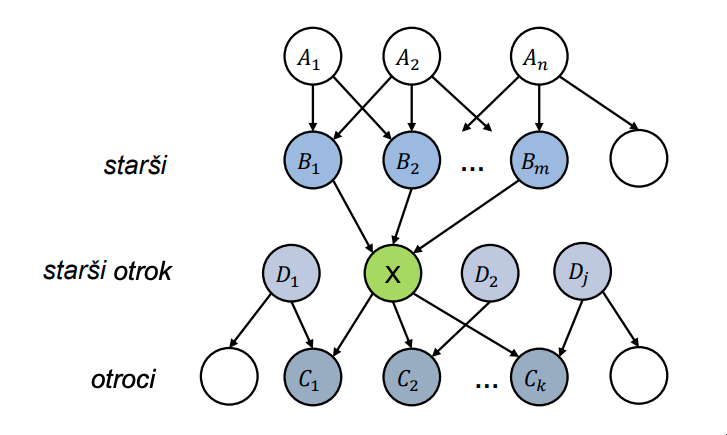
\includegraphics[width=3cm]{images/ovojnica-markova.png}
\subsection{D-locevanje}
A in B v mrezi sta \textbf{neodvisni} $\Leftrightarrow$ obstaja mnozica vozlisc E, ki d-locuje A in B, potem sledi:  (\green{$P(A|EB)=P(A|E)$})\\
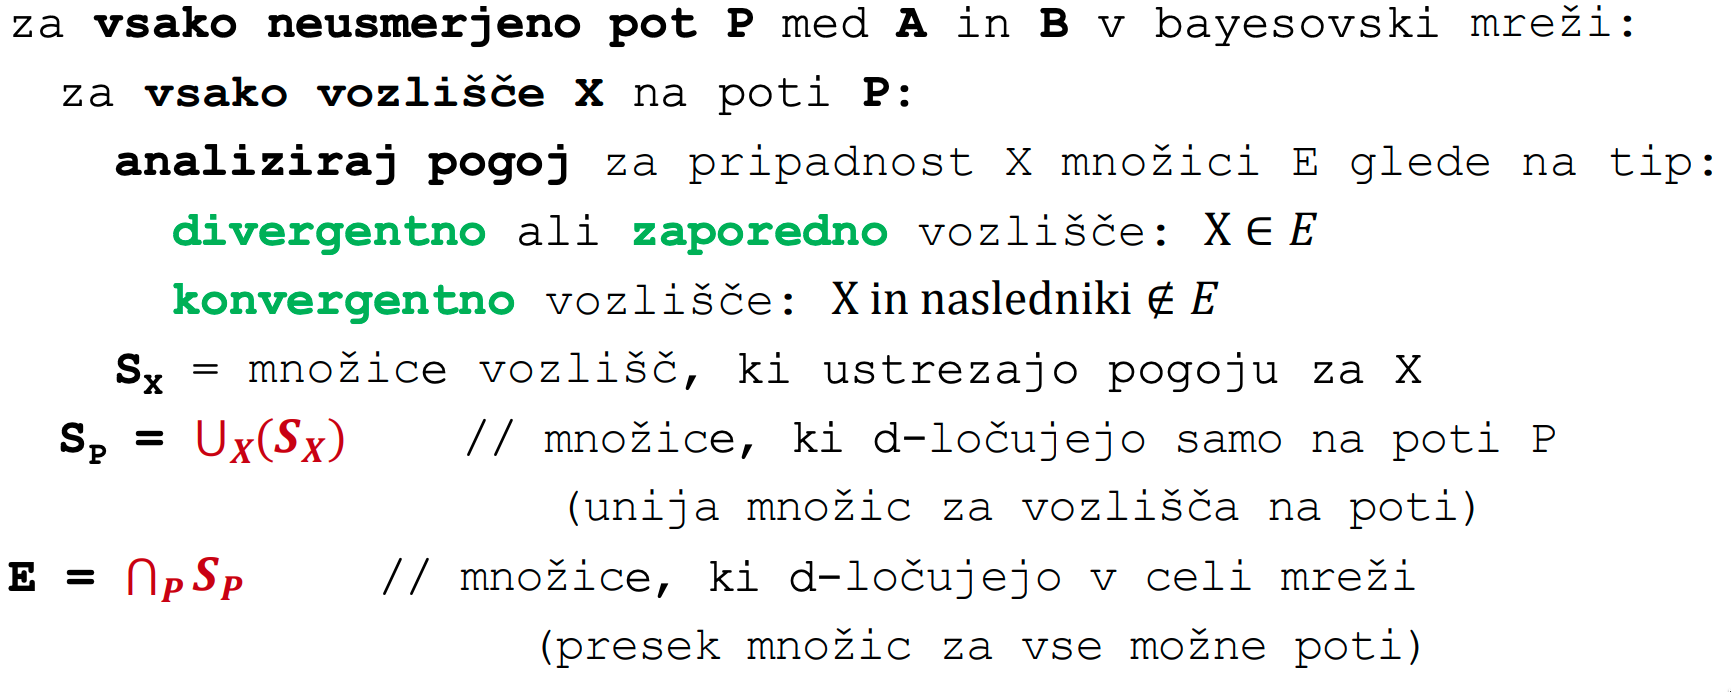
\includegraphics[width=6.5cm]{images/d-locevanje-algoritem.png}
\includegraphics*[width=7cm]{images/d-locevanje-nacini.png}
\red{! pri konvergentnem izlocimo tudi vse naslednike X}\\
Primer d-locevanje vozlisc c in d\\
\includegraphics*[width=6cm]{images/primer-d-locevanje.png}\\
$\rightarrow$ P(d|c\blue{a})=P(d|a), P(d|c\blue{b})=P(d|b), P(d|c\blue{ab})=P(d|ab),\\
P(d|c\blue{be})=P(d|be),P(d|c\blue{abe})=P(d|abe)
\subsection{I-ekvivalentnost}
Mrezi sta \green{I-ekvivalentni} ce imate \textbf{enako strukturo} (ob ignoriranju usmerjenosti povezav) in \textbf{ista konvergentna vozlisca}:\\
\includegraphics*[width=7cm]{./images/i-ekvivalentnost.png}